\chapter{Hintergrund}\label{ch:hintergrund}
Im Folgenden wird das Konzept des \textit{kontextzentrischen sozialen Netzes} erläutert, das dieser Arbeit zu Grunde liegt. Anschließend werden mengentheoretische und probabilistische Grundlagen und Verfahren sowie Daten- und Indexstrukturen dargestellt, die Eingang in diese Arbeit gefunden haben. Es wird erläutert, inwiefern sie für das soziale Online-Netz AMBIENCE relevant sind oder darin verwendet werden. 
\section{Kontextzentrische soziale Netze}\label{sec:kontext}
Mit Zunahme der mobilen Endgeräte und dem Erfolgszug des Smartphones lässt sich eine Tendenz beobachten, die von bestehenden sozialen Online-Netzwerken wenig abgebildet wird: Weg von adressbasiertem Routing und Ende-zu-Ende-Kommunikation hin zu \textit{context-awareness} und \textit{information-centric networking}. 

Der Begriff context-awareness wurde von Schilit et al. 1994 geprägt und bezeichnet die Nutzung von Kontextinformationen als Informationsquelle für Anwendungen und Netzwerke \cite{Schilit1994}. Information-centric networking (ICN) bezeichnet ein neuartiges Konzept für Netzwerke, die nicht auf Ende-zu-Ende- oder Sender/Empfänger-Kommunikation basieren, sondern auf den im Netzwerk vorhandenen Informationen \cite{Ahlgren2012}. 
Der Begriff \textit{Kontext} im Zusammenhang mit interaktiven Anwendungen wurde bereits in den 90er Jahren geprägt. Die klassische Definition von Dey und Abowd lautet: 
\begin{quote}
\textit{"`Context is any information that can be used to characterize the situation of an entity. An entity is a person, place, or object that is considered relevant to the interaction between a user and an application including the user and application themselves."'} \cite{Dey1999} 
\end{quote}
Diese Definition lässt sich für soziale Online-Netze eingrenzen auf 
\begin{quote}
\textit{"`[...] any information that can be used to infer aspects of the surroundings of an entity in a way, in which some applications may have interest. Surroundings include all information that could possibly impact the behaviour of the entity."'} \cite{Werner2015}
\end{quote}
Ein kontextzentrisches soziales Netz ist also ein soziales Online-Netz, das auf Kontext-Variablen wie Ort und Zeit als Informationsquellen basiert und in der Regel dezentral organisiert ist, z.B. durch eine Peer-to-Peer- statt einer Client/Server-Architektur. Kommunikation beruht darin allein auf Kontext-Ähnlichkeit, nicht auf Online-Freundschaft: 
\begin{quote}
\textit{"`A context-centric online social network is an online social network in which the edges of the social graph are defined from context information and context matching algorithms. An edge between two profiles exists for a fixed information object if and only if the two profiles share the relevant context as defined by the publisher."'} \cite{Werner2015}
\end{quote}
\paragraph*{AMBIENCE}
AMBIENCE ist ein soziales Online-Netzwerk, das 2015 als Prototyp implementiert wurde und sich an diesem neuen Paradigma orientiert. Die vorliegende Arbeit hat das Ziel, einen spezifischen Aspekt des Netzwerks zu optimieren, nämlich die Organisation der Nachrichten für \textit{k}-nächste-Nachbarn-Anfragen an einen Host. Nachrichten und Anfragen werden in AMBIENCE als Bloom-Filter kodiert. Bei einer Anfrage wird also ein Anfrage-Filter mit einer Menge von Bloom-Filtern verglichen, die an einem Host gespeichert sind. Aktuell werden die Filter dort einfach als unsortierte Liste gespeichert. Die Laufzeit für \textit{k}-nächste-Nachbarn-Anfragen an einen Host mit \textit{n} Filtern liegt damit in $O(n^2)$. Dieses Laufzeitverhalten gilt es zu optimieren, wenn das Netzwerk wachsen und über den Status eines Prototypen hinaus erfolgreich sein soll. 
\section{Bloom-Filter}\label{sec:bloom}
Ein Bloom-Filter ist eine probabilistische Datenstruktur zur Beschreibung von Mengen und wurde in der ursprünglichen Form 1970 von Burton H. Bloom eingeführt \cite{Bloom1970}. Er besteht aus einem Bit-Array der festen Länge \textit{m}, dessen Elemente zunächst alle auf 0 gesetzt sind. Das Einfügen von Informationsobjekten basiert auf der Berechnung einer festen Anzahl unabhängiger Hashfunktionen \textit{k}, die positive Werte kleiner als \textit{m} annehmen. Soll ein Objekt in den Filter eingefügt werden, werden seine Hashwerte berechnet und die entsprechenden Bits im Filter gesetzt \cite{Broder2004}. 

Die Hashwerte werden für Anfragen an den Filter verwendet. Ist ein Objekt im Filter enthalten, sind seine charakteristischen Bits gesetzt worden, d.h. man kann eine Anfrage nach seinen Hashwerten durchführen und mit großer Wahrscheinlichkeit ermitteln, ob es im Filter vorhanden ist. Sind ein oder mehrere Bits des Anfrageobjekts nicht gesetzt, ist es mit Sicherheit nicht im Filter vorhanden. Es gibt also keine falsch negativen Antworten. Allerdings kann es sein, dass ein Element nicht in den Filter eingefügt wurde, obwohl alle seine Bits gesetzt sind (falsch positive Antworten). Grund dafür ist die Kollisionseigenschaft von Hashfunktionen, die ein großes Universum von Objekten auf einen sehr viel kleineren Wertebereich, hier die Länge des Bloom-Filters, abbilden. Es kann somit zu Kollisionen zwischen unterschiedlichen Informationsobjekten bzw. ihren charakteristischen Hashwerten kommen. 

Die Falsch-Positiv-Rate eines Bloom-Filters ist abhängig von \textit{m}, \textit{k} und der Anzahl der eingefügten Elemente \textit{n}. Dieser Zusammenhang ist von zentraler Bedeutung, um die Vorteile von Bloom-Filtern richtig nutzen zu können. Die Falsch-Positiv-Rate lässt sich wie folgt bestimmen \cite{Broder2004}: 

Nach dem Einfügen aller Objekte in den Filter beträgt die Wahrscheinlichkeit dafür, dass ein beliebiges Bit den Wert 0 hat, 
\[\left(1 - \frac{1}{m}\right)^{kn}\approx e^{-kn/m}.\]
Unter der Voraussetzung optimaler, zufälliger Hashfunktionen darf man $p = e^{-kn/m}$ annehmen und erhält für die Falsch-Positiv-Rate
\[f = \left(1 - \left(1-\frac{1}{m}\right)^{kn}\right)^k\approx\left(1 - e^{-kn/m}\right)^k = (1-p)^k.\]

Das bedeutet: Die Falsch-Positiv-Rate eines Bloom-Filters steigt mit der Anzahl der eingefügten Objekte und der Anzahl der verwendeten Hashfunktionen, die zum Einfügen jedes Objekts verwendet werden, und sinkt mit steigender Größe des Daten-Arrays im Bloom-Filter. Offensichtlich sind also drei Performanz-Metriken im Bloom-Filter von Bedeutung, die mit Hilfe der Parameter \textit{m}, \textit{k} und \textit{f} beeinflusst werden können: Filtergröße, Geschwindigkeit und Falsch-Positiv-Rate.  

Abhängig vom Anwendungsfall kann der Anwender also entscheiden, welche Metrik(en) für den Bloom-Filter optimiert werden sollen. Werden Bloom-Filter zur Übermittlung von Nachrichten in einem Verteilten System genutzt, wird man womöglich eine höhere Falsch-Positiv-Rate zu Gunsten einer kleineren Nachrichtenlänge bzw. Filtergröße in Kauf nehmen \cite{Mitzenmacher2002}. In einem Datenbank-Managementsystem wird man hingegen versuchen, die Falsch-Positiv-Rate möglichst niedrig zu halten, da jeder Zugriff auf den Sekundärspeicher rechen- und zeitaufwändig ist. Es liegt also nahe, falsch positive Ergebnisse und damit überflüssige Plattenzugriffe möglichst zu vermeiden. Wieder andere Anwendungen müssen möglichst schnell Ergebnisse liefern wie z.B. der Abgleich mit einer schwarzen Liste von Webseiten. Wird eine Webseite auf Grund eines falsch positiven Ergebnisses versehentlich als bösartig eingestuft, obwohl sie keinen schädlichen Inhalt hat, ist dies sicherlich eher zu tolerieren als ein unverhältnismäßig hoher Zeitaufwand für den Abgleich. In diesem Fall würde man vermutlich eher die Filtergröße reduzieren, um rasch ein Suchergebnis zu erhalten, und eine erhöhte Falsch-Positiv-Rate in Kauf nehmen. 

Aus der Kollisionseigenschaft folgt auch, dass ein einmal eingefügtes Objekt nicht mehr aus einem Bloom-Filter entfernt werden kann. Das könnte offensichtlich zu falsch negativen Ergebnissen für andere Objekte führen. Abbildung \ref{fig:pic0} zeigt ein Beispiel für einen Bloom-Filter, in den die Objekte \textit{x}, \textit{y} und \textit{z} eingefügt wurden. Das Objekt \textit{w} ist nicht im Filter vorhanden\footnote{Bildnachweis: \url{https://commons.wikimedia.org/wiki/File:Bloom_filter.svg} (17.07.2016).}.
\begin{figure}[hpbt]
  \centering
  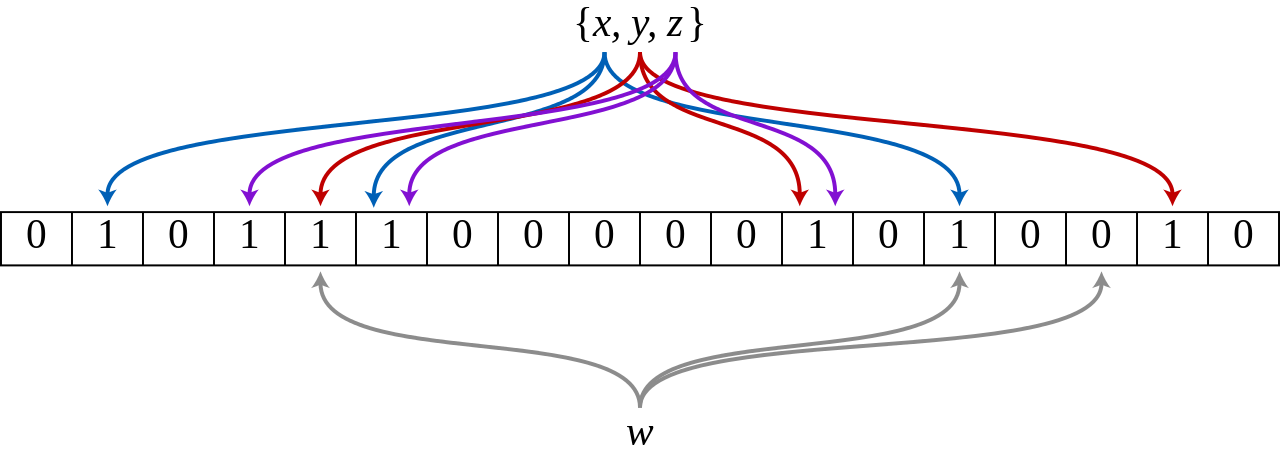
\includegraphics[width=0.8\textwidth]{pictures/1280px-Bloom_filter.png}\\
  \caption[Bloom-Filter]{Bloom-Filter.}\label{fig:pic0}
\end{figure}
\subsection{Distanzmaße}\label{sec:distanzmasse}
Um die Ähnlichkeit zweier Mengen zu ermitteln, werden unterschiedliche Distanzmetriken oder Ähnlichkeitsmaße verwendet. Für den Vergleich von Bloom-Filtern und insbesondere für die \textit{k}-nächste-Nachbarn-Suche muss ein geeignetes Ähnlichkeitsmaß zur Anwendung kommen. Bayardo et al. verwenden dazu die \textit{Kosinus-Ähnlichkeit} \cite{Bayardo2007}, Sakuma und Sato definieren die Ähnlichkeit von Bloom-Filtern als die Anzahl gleicher 1-Bits \cite{Sakuma2011}. Ist diese für zwei Filter identisch, werden die Bit-Arrays negiert und die Anzahl gleicher 0-Bits ermittelt. 

In AMBIENCE wird eine Abschätzung der \textit{Jaccard-Distanz} zur Ermittlung der Ähnlichkeit von Bloom-Filtern verwendet. Die Jaccard-Distanz zwischen zwei Mengen \textit{A} und \textit{B} ist definiert als 
\[J_{\delta}(A,B) = 1 - J(A,B) = \frac{|A\cap B| - |A\cup B|}{|A\cup B|}, \]
wobei 
\[J(A,B) = \frac{|A\cap B|}{|A\cup B|}\] den \textit{Jaccard-Koeffizienten} bezeichnet. Die Jaccard-Distanz nimmt Werte im Bereich $\left[0,1\right]$ an. Identische Mengen haben eine Jaccard-Distanz von 0, Mengen ohne gemeinsame Elemente haben eine Jaccard-Distanz von 1. 
Für Bloom-Filter lässt sich die Jaccard-Distanz analog berechnen. Die Vereinigungsmenge zweier Bloom-Filter \textit{F} und \textit{G} lässt sich als bitweises logisches Oder, die Schnittmenge als bitweises logisches Und repräsentieren. Auch hier nimmt die Jaccard-Distanz offensichtlich Werte zwischen 0 und 1 an. Je ähnlicher die Filter sind, desto kleiner ist ihre Jaccard-Distanz. 
Die Jaccard-Distanz zwischen Bloom-Filtern ist, anders als die von Sakuma und Sato verwendete Distanzmetrik, nicht transitiv in dem Sinne, dass zwei Filter, die beide eine geringe Jaccard-Distanz zu einem dritten Filter aufweisen, untereinander nicht ähnlich sein müssen. Man betrachte z.B. die Filter \textit{F1}, \textit{F2} und \textit{F3} (vgl. Abbildung \ref{fig:pic1}).  
\begin{figure}
  \centering
  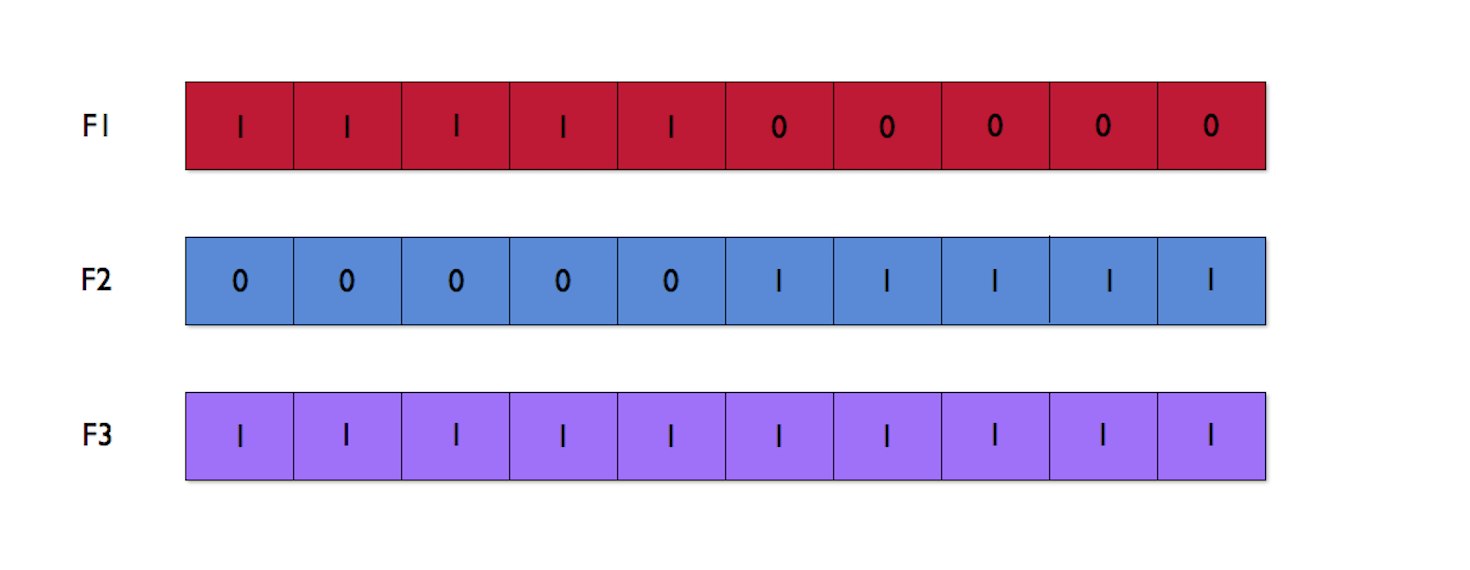
\includegraphics[width=1.0\textwidth]{pictures/filters.png}\\
  \caption[Jaccard-Distanzen zwischen Bloom-Filtern]{Jaccard-Distanzen zwischen Bloom-Filtern.}\label{fig:pic1}
\end{figure}
\noindent
Die Jaccard-Distanzen zwischen \textit{F1}, \textit{F2} und \textit{F3} betragen: 
\[J_{\delta}(F1,F3) = 1 - J(F1,F3) = 1 - \frac{|F1\cap F3|}{|F1\cup F3|} = 1 - \frac{5}{10} = 0.5\]
\[J_{\delta}(F2,F3) = 1 - J(F2,F3) = 1 - \frac{|F2\cap F3|}{|F2\cup F3|} = 1 - \frac{5}{10} = 0.5\]
\[J_{\delta}(F1,F2) = 1 - J(F1,F2) = 1 - \frac{|F1\cap F2|}{|F1\cup F2|} = 1 - 0 = 1\]
Daran wird deutlich: Obwohl \textit{F1} und \textit{F2} jeweils die Hälfte der Elemente mit \textit{F3} gemeinsam haben, lässt sich daraus kein Wert für die Ähnlichkeit zwischen \textit{F1} und \textit{F2} ableiten. Sie sind sich im Gegenteil maximal unähnlich. 
\subsection{Teil- und Obermengenbeziehung}\label{sec:mengenbeziehungen}
Will man Bloom-Filter z.B. nach Ähnlichkeit gruppieren, kann man stattdessen Teil- und Obermengenbeziehungen zwischen ihnen betrachten. Die Teilmengenbeziehung zwischen zwei Bloom-Filtern sei hier wie folgt definiert: 
\begin{quote}
Ein Bloom-Filter \textit{F} ist \textit{Teilmenge} eines Bloom-Filters \textit{G}, wenn darin mindestens die gleichen 0-Bits gesetzt sind wie in \textit{G} (und möglicherweise weitere, zusätzliche 0-Bits).
\end{quote}
Die Obermengenbeziehung zwischen zwei Bloom-Filtern sei hier wie folgt definiert: 
\begin{quote}
Ein Bloom-Filter \textit{F} ist \textit{Obermenge} eines Bloom-Filters \textit{G}, wenn darin mindestens die gleichen 1-Bits gesetzt sind wie in \textit{G} (und möglicherweise weitere, zusätzliche 1-Bits).
\end{quote}
Der maximal gefüllte Filter, in dem alle Bits gesetzt sind, ist damit Obermenge aller Filter derselben Länge (auch von sich selbst). Der leere Filter ist die (triviale) Teilmenge aller Filter derselben Länge (auch von sich selbst). Teil- und Obermengen sind Umkehrungen voneinander, d.h. wenn \textit{F} Teilmenge von \textit{G} ist, folgt daraus, dass \textit{G} Obermenge von \textit{F} ist, und umgekehrt.  

Zwischen den Bloom-Filtern in Abbildung \ref{fig:pic1} bestehen folgende Teil- und Obermengenbeziehungen: \textit{F1} und \textit{F2} sind Teilmengen von \textit{F3}. \textit{F3} ist Obermenge von \textit{F1} und \textit{F2}. Zwischen den maximal unähnlichen Filtern \textit{F1} und \textit{F2} bestehen keine Teil- und Obermengenbeziehungen. 
\begin{figure}[hpbt]
  \centering
  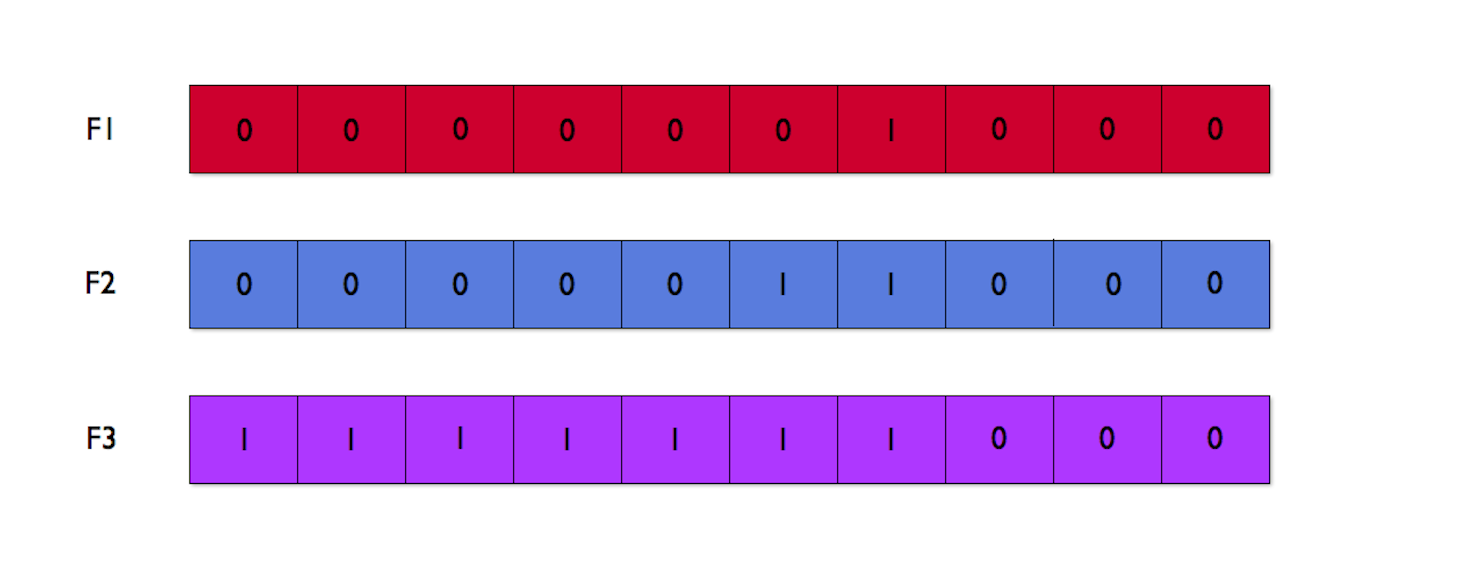
\includegraphics[width=1.0\textwidth]{pictures/distances.png}\\
  \caption[Teil- und Obermengenbeziehungen zwischen Bloom-Filtern]{Teil- und Obermengenbeziehungen zwischen Bloom-Filtern.}\label{fig:pic2}
\end{figure}

\noindent
Teil- und Obermengenbeziehung sind außerdem transitiv, was an Abbildung \ref{fig:pic2} deutlich wird: \textit{F1} ist Teilmenge von \textit{F2}, damit auch Teilmenge von \textit{F3}. \textit{F3} ist Obermenge von \textit{F2}, damit auch Obermenge von \textit{F1}. 

Teil- und Obermengenbeziehungen sind also im Gegensatz zur Jaccard-Distanz dazu geeignet, transitive Ähnlichkeitsbeziehungen zwischen Bloom-Filtern abzubilden. Diese Eigenschaft spielt eine zentrale Rolle im hier entwickelten Verfahren, das in Kapitel \ref{ch:implementierung} ausführlich dargestellt wird. 
\subsection{Hashfunktionen}\label{sec:hashfunktionen}
Zum Einfügen von Objekten in einen Bloom-Filter werden \textit{k} unabhängige Hashfunktionen $h_1,\ldots , h_k$ mit Wertebereich $\{ 0,\ldots, m-1\}$ verwendet, wobei \textit{m} die Größe des Bloom-Filters bezeichnet. Dabei wird davon ausgegangen, dass diese Hashfunktionen jedem Objekt im Universum einen zufälligen Hashwert aus dem Bereich $\{ 0,\ldots, m-1\}$ zuweisen, und dass diese Werte einer Gleichverteilung folgen \cite{Mitzenmacher2002}. Die optimale Anzahl an Hashfunktionen, die zur Minimierung der Falsch-Positiv-Rate benötigt wird, lässt sich in Abhängigkeit von den Parametern \textit{m}, \textit{n} und \textit{f} berechnen. Hierbei bezeichnet \textit{m} die Filtergröße, \textit{n} die Anzahl der erwarteten einzufügenden Objekte und \textit{f} die maximal akzeptierte Falsch-Positiv-Rate. Damit lässt sich die Anzahl benötigter Bits, d.h. die Filtergröße, berechnen als
\[m = -n\ast ln(f) / (ln(2)^2).\]
Hat man die Filtergröße bestimmt, lässt sich die Anzahl benötigter Hashfunktionen berechnen als 
\[d = \Ceil[\Bigg]{\frac{m}{n}\ast ln(2)}.\]
Die Frage nach den idealen Hashfunktionen für einen Bloom-Filter ist nicht eindeutig zu beantworten \cite{Broder2004}. Grundsätzlich muss zwischen kryptografischen Hashfunktionen wie MD5 und SHA und gewöhnlichen Hashfunktionen wie Murmur- oder Jenkins-Hashfunktionen unterschieden werden. Die Berechnung von kryptografischen Hashfunktionen dauert in der Regel länger, dafür haben sie bestimmte Eigenschaften wie eine hohe Kollisionsresistenz und Gleichverteilung der Ergebniswerte. 

Werden Bloom-Filter z.B. zum schnellen Nachschlagen in großen, verteilten Datenbanken eingesetzt, wird auf die kryptografischen Eigenschaften zu Gunsten des verminderten Rechenaufwandes verzichtet. Das NoSQL-Datenbanksystem Cassandra und das Hadoop-Framework für skalierte, verteilt arbeitende Software verwenden beispielsweise Bloom-Filter in Kombination mit Murmur- und Jenkins-Hashfunktionen. Darüber hinaus ist MD5 für Bloom-Filter weit verbreitet. Murmur-Hashfunktionen haben gute Verteilungseigenschaften und lassen sich vergleichsweise schnell berechnen, weswegen sie generell für den Einsatz in Bloom-Filtern empfohlen werden\footnote{Vgl. \mbox{\url{http://spyced.blogspot.de/2009/01/all-you-ever-wanted-to-know-about.html} (17.07.2016).}}. AMBIENCE verwendet Murmur-Hashfunktionen zur Generierung der Bloom-Filter. Für die eigene Implementierung wurde der Murmur2-Hash verwendet\footnote{Vgl. \url{https://sites.google.com/site/murmurhash/MurmurHash2.cpp} (17.07.2016) für den Quellcode.}.  
\subsection{Bloom-Filter-Varianten und Anwendungen}\label{sec:bloom-anwendungen}
Wegen ihres geringen Speicherbedarfs und einfachen Implementierung erfreuen sich Bloom-Filter in unterschiedlichsten Versionen großer Beliebtheit. Wichtige Varianten sind z.B. \textit{Attenuated Bloom Filter}, \textit{Counting Bloom Filter} und \textit{Compressed Bloom Filter}. Ein Counting Bloom-Filter benötigt mehr Speicherplatz als ein klassischer Bloom-Filter, dafür können Objekte wieder daraus entfernt werden \cite{Fan2000}. Komprimierte Bloom-Filter werden eingesetzt, wenn Bloom-Filter als Nachrichten mit begrenzter Länge versendet werden oder die übertragene Datenmenge minimiert werden soll \cite{Mitzenmacher2002}. Attenuated Bloom-Filter \cite{Sakuma2011} können als Array von Bloom-Filtern betrachtet werden und können z.B. in einem Netzwerk Informationen darüber enthalten, welche Dienste an einem anderen Knoten verfügbar sind. Besonders häufig kommen Bloom-Filter in verteilten Anwendungen und Netzwerkdiensten zum Einsatz \cite{Broder2004}. 

Neben Hadoop und Cassandra werden Bloom-Filter in unzähligen, zum Teil hoch skalierenden Anwendungen eingesetzt. Weitere Beispiele sind der quelloffene Webproxy Squid und der Chrome-Browser, wo Bloom-Filter zum schnellen Nachschlagen von als bösartig eingestuften URLs verwendet werden. Broder und Mitzenmacher formulieren das Bloom-Filter-Prinzip wie folgt: 
\begin{quote}
\textit{"`Wherever a list or set is used, and space is at a premium, consider using a Bloom filter if the effect of false positives can be mitigated."'} \cite{Broder2004}
\end{quote}
\section{Indexstrukturen}\label{sec:indexstrukturen}
Zur effizienten Bearbeitung von Anfragen und Operationen kommen in der internen Schicht von Datenbanksystemen spezielle Datenstrukturen und Speicherverfahren zum Einsatz. Sie werden \textit{Indexstrukturen} genannt und organisieren die Daten an Hand von Indizes, um die gewünschten Operationen zu unterstützen.\footnote{Trotz der großen Verbreitung von Indexstrukturen in Datenbanksystemen scheinen in der Literatur keine überblicksartigen Darstellungen zu existieren. Der aktuelle Abschnitt stützt sich daher im Wesentlichen auf das Skript zur Vorlesung \textit{Anfragebearbeitung und Indexstrukturen in Datenbanksystemen} im Wintersemester 2013/2014 an der Ludwig-Maximilians-Universität München \cite{Kriegel1994--2013}.}

Ein \textit{Index} oder \textit{Verzeichnis} einer Datei enthält Informationen über ihre Struktur, wobei mit "`Datei"' in diesem Zusammenhang eine komplette Datenstruktur gemeint ist, also z.B. ein Suchbaum oder ein Array. Den Datensätzen werden dabei meist Schlüssel oder IDs zugewiesen, an Hand derer sie in der Indexstruktur organisiert und gesucht werden. D.h. nicht die Datensätze selbst werden einer einer bestimmten Ordnung zu Folge organisiert, sondern lediglich ihre Schlüssel. Eine Anfrage nach einem Datensatz ermittelt dann zunächst den zugehörigen Schlüssel, sucht dessen Position in der Indexstruktur und greift erst dann auf den tatsächlichen Datensatz zu, wenn seine Position z.B. auf dem Plattenspeicher ermittelt wurde. Indexstrukturen lassen sich danach klassifizieren, wie sie die Daten organisieren: 
\begin{enumerate}
\setlength{\itemsep}{20pt}
	\item \textit{Daten-organisierende Indexstrukturen} werden zur Organisation der tatsächlich anfallenden Daten eingesetzt -- meist in Form von \textit{Suchbäumen}. 
	\item \textit{Raum-organisierende Indexstrukturen} werden zur Organisation des Speichers eingesetzt, in dem die Daten gehalten werden. Sie verwenden vor allem \textit{dynamische Hashverfahren}. 
	\item \textit{Hybride Indexstrukturen} sind eine Kombination der vorgenannten Klassen und basieren auf \textit{Hashbäumen}.   
\end{enumerate}
% \enlargethispage{2\baselineskip}
Eine gute bzw. effektive Indexstruktur sollte folgenden Anforderungen genügen: 
\begin{enumerate}
\setlength{\itemsep}{20pt}
	\item \textit{Effiziente Suche:} Eine Suchanfrage auf der Indexstruktur soll in optimaler Zeit ein Ergebnis liefern. D.h. die Anfrage soll in möglichst wenigen Schritten an die Seite oder Seiten weiter geleitet werden, die die angefragten Daten enthalten.
	\item \textit{Dynamisches Einfügen, Modifizieren und Löschen von Datensätzen:} Die zu organisierende Datenmenge verändert sich möglicherweise über die Zeit, was durch die Indexstruktur widergespiegelt und unterstützt werden muss.  
	\item \textit{Erhalt der lokalen Ordnung:} Falls es Datensätze gibt, deren Schlüssel in der angewandten Ordnungsrelation (z.B. die Kleiner-Gleich-Ordnung) aufeinander folgen, sollte die Indexstruktur diese Ordnung übernehmen. Suchbäumen erfüllen diese Eigenschaft, nicht aber lineare Hashverfahren. Die Wahl bzw. Implementierung der Indexstruktur muss also zum Anwendungsfall passen. 
	\item \textit{Speichereffizienz:} Effiziente Speichernutzung ist für real existierende und hoch skalierende Anwendungen von zentraler Bedeutung. 
\end{enumerate}
Weitere mögliche Anforderungen sind \textit{Machbarkeit} und \textit{Implementierungskosten}. Sie sind für die vorgestellte Implementierung nachrangig in dem Sinne, dass der Nachweis der Machbarkeit durch die Implementierung selbst erfolgt. Da AMBIENCE ein Prototyp ist und im akademischen Umfeld entwickelt wurde, kann die wirtschaftliche Kalkulation der Kosten, wie sie ein Unternehmen vornehmen würde, außer Acht gelassen werden. 

Für Implementierung (vgl. Kapitel \ref{ch:implementierung}) und Evaluation (vgl. Kapitel \ref{ch:evaluation}) stehen daher die Anforderungen 1--4 im Mittelpunkt. Als weiteres Kriterium, das nicht zu den allgemeinen Anforderungen an Indexstrukturen zählt, wurden die Aufbaukosten der Indexstruktur betrachtet. 
\subsection{B-Bäume}\label{sec:b-bäume}
B-Bäume sind eine weit verbreitete Form der Suchbäume und wurden zuerst 1972 von Rudolf Bayer und Edward M. McCreight vorgestellt. Sie erfüllen unter anderem folgende Eigenschaften:  
\begin{enumerate}
\setlength{\itemsep}{20pt}
	\item \textit{Aufbau:} B- und B$^+$-Bäume wachsen und schrumpfen von der Wurzel ausgehend.
	\item \textit{Balanciertheit:} Alle Blätter sind auf demselben Level. 
	\item \textit{Minimaler Grad/Ordnung:} B- und B$^+$-Bäume sind definiert durch die Ordnung oder den minimalen Grad \textit{t}, d.h. jeder Knoten außer der Wurzel enthält mindestens \textit{t} Schlüssel. 
	\item \textit{Suchbaumeigenschaft:} Schlüssel sind aufsteigend sortiert.
	\item \textit{Verzweigungsgrad:} Ein innerer Knoten mit \textit{k} Schlüsseln hat genau \textit{k+1} Kinder \cite{Ottmann2012}. Den Grad bzw. die minimale Ordnung betreffend ist die Nomenklatur in der Literatur uneinheitlich. Ottmann und Widmeyer \cite{Ottmann2012} sprechen in sprechen in Anlehnung an Knuth \cite{Knuth1999} von B-Bäumen der Ordnung \textit{m} und fordern, dass jeder Knoten mit Ausnahme der Wurzel und der Blätter mindestens $\lceil\frac{m}{2}\rceil$ Schlüssel enthalte. Stein et al. definieren den minimalen Grad wie weiter oben beschrieben \cite{Stein2009}, Kriegel verwendet dasselbe Kriterium, bezeichnet es jedoch als Grad \textit{m} \cite{Kriegel1994--2013}.
\end{enumerate}	
Abbildung \ref{fig:pic3} zeigt einen B-Baum der Ordnung 2, in den die Schlüssel \textbf{A--G}, \textbf{I--M}, \textbf{O--T}, \textbf{V--X} und \textbf{Z} eingefügt wurden. Ordnung 2 bedeutet: Die Wurzel muss mindestens einen Schlüssel enthalten, in diesem Fall den Wert \textbf{K}. Jeder innere Knoten und jedes Blatt enthält mindestens zwei Schlüssel. Der Verzweigungsgrad eines inneren Knotens ist um eins größer als die Anzahl seiner Schlüssel, z.B. hat die Wurzel einen Schlüssel und zwei Kindknoten. Alle Blätter sind auf demselben Level, in diesem Fall auf Level 3. Die Suchbaumeigenschaft ist erfüllt, d.h. der Schlüssel mit dem lexikografisch kleinsten Wert \textbf{A} ist am weitesten links, der Schlüssel mit dem lexikografisch größten Wert \textbf{Z} ist am weitesten rechts im Baum zu finden. 
\begin{figure}[hpbt]
  \centering
  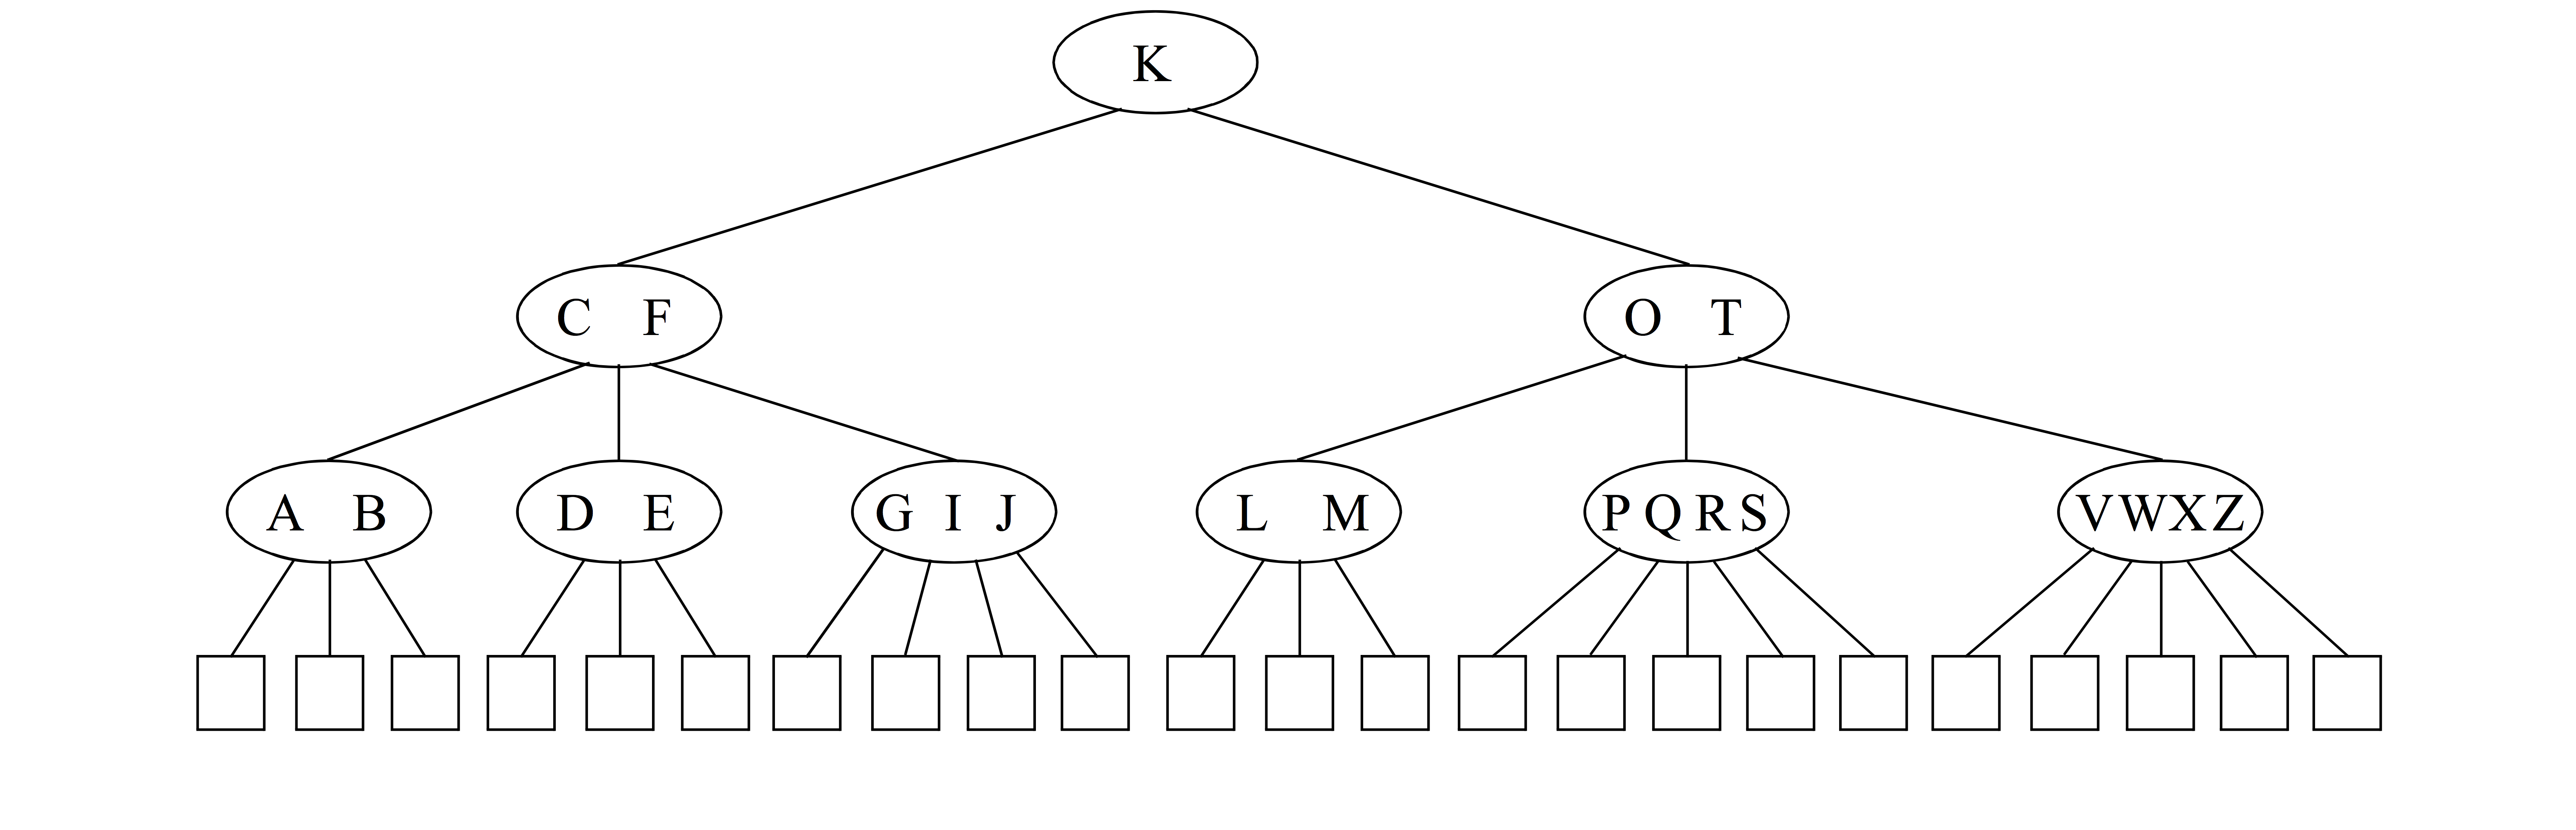
\includegraphics[width=1.0\textwidth]{pictures/b-baum.png}\\
  \caption[Ein B-Baum der Ordnung 2]{Ein B-Baum der Ordnung 2 \cite{Kriegel1994--2013}.}\label{fig:pic3}
\end{figure}
Unterstützte Operationen sind in der Regel Einfügen, Suchen und Löschen von Datensätzen. Dabei ist die Löschoperation am aufwendigsten zu implementieren, da auch das Löschen eines Schlüssels aus einem inneren Knoten betrachtet werden muss. Ein Schlüssel aus einem inneren Knoten kann nicht direkt gelöscht werden, da er zusätzlich als Separator für seine Kindknoten dient. Es muss daher ein neuer Separator aus dem rechten oder linken Kindknoten entnommen und in den Knoten eingefügt werden. Falls damit die B-Baum-Eigenschaften verletzt werden, d.h. der Kindknoten anschließend zu wenig Schlüssel enthält, muss eine Underflow-Behandlung eingeleitet werden, bei dem der Kindknoten mit einem Geschwisterknoten verschmolzen wird. Der Underflow kann sich rekursiv bis zur Wurzel fortsetzen und dafür sorgen, dass der Baum eine Ebene verliert und eine neue Wurzel erhält. 
\subsection{B$^+$-Bäume}\label{sec:b+bäume}
Das entwickelte Verfahren stützt sich stark auf \textit{B$^+$-Bäume}, eine Erweiterung der B-Bäume. Sie unterscheiden sich von ihnen in folgenden Eigenschaften: 
\begin{enumerate}
\setlength{\itemsep}{20pt}
	\item \textit{Minimale Schlüsselanzahl:} Jeder innere Knoten enthält mindestens einen Schlüssel.  
	\item \textit{Ordnungsrelation:} Der Kindknoten zwischen den Schlüsseln \textit{k1} und \textit{k2} enthält alle Schlüssel $\geq$ \textit{k1} und < \textit{k2}.
	\item \textit{Speicherung der Datensätze:} Alle Schlüssel werden auch in den Blättern gespeichert. Die tatsächlichen Datensätze sind mit dem entsprechen Schlüssel im Blatt verknüpft. 
	\item \textit{Sequentielle Verkettung:} Alle Blätter sind gemäß der Ordnung auf den Primärschlüsseln verkettet. 
\end{enumerate}
Abbildung \ref{fig:pic4} zeigt einen B$^+$-Baum der Ordnung 2, in den die Schlüssel \textbf{An}, \textbf{And}, \textbf{Certain}, \textbf{For}, \textbf{From}, \textbf{Which} und \textbf{With} eingefügt wurden. Ordnung 2 bedeutet in diesem Fall: Die Wurzel muss mindestens einen Schlüssel enthalten, in diesem Fall den Wert \textbf{For}. Jeder innere Knoten enthält mindestens einen und jedes Blatt enthält mindestens zwei Schlüssel. Der Verzweigungsgrad eines inneren Knotens ist um eins größer als die Anzahl seiner Schlüssel, z.B. hat die Wurzel einen Schlüssel und zwei Kindknoten. Alle Blätter sind auf demselben Level, in diesem Fall auf Level 3.

Die inneren Baumknoten erfüllen die Ordnungsrelation \textit{k1} < Kindknoten-Schlüssel $\leq$ \textit{k2}. Z.B. enthält der Blattknoten ganz links alle Schlüssel, deren Wert lexikografisch kleiner ist als der \textbf{Certain} im Elternknoten. Der zweite Blattknoten enthält alle Schlüssel, deren Wert lexikografisch $\geq$ \textbf{Certain} ist und zudem kleiner als \textbf{For}, den Schlüssel im Wurzelknoten, da die Ordnungsrelation natürlich im ganzen Baum erfüllt sein muss. Alle Datensätze sind auch in den Blättern gespeichert, z.B. findet sich der Schlüssel \textbf{For} sowohl in der Wurzel als auch im dritten Blattknoten. Darin unterscheidet sich der B$^+$-Baum vom B-Baum. Dort ist der Schlüssel \textbf{K} z.B. nur in der Wurzel abgespeichert, nicht aber im Blattknoten (vgl. Abbildung \ref{fig:pic3}).  
\begin{figure}[hpbt]
  \centering
  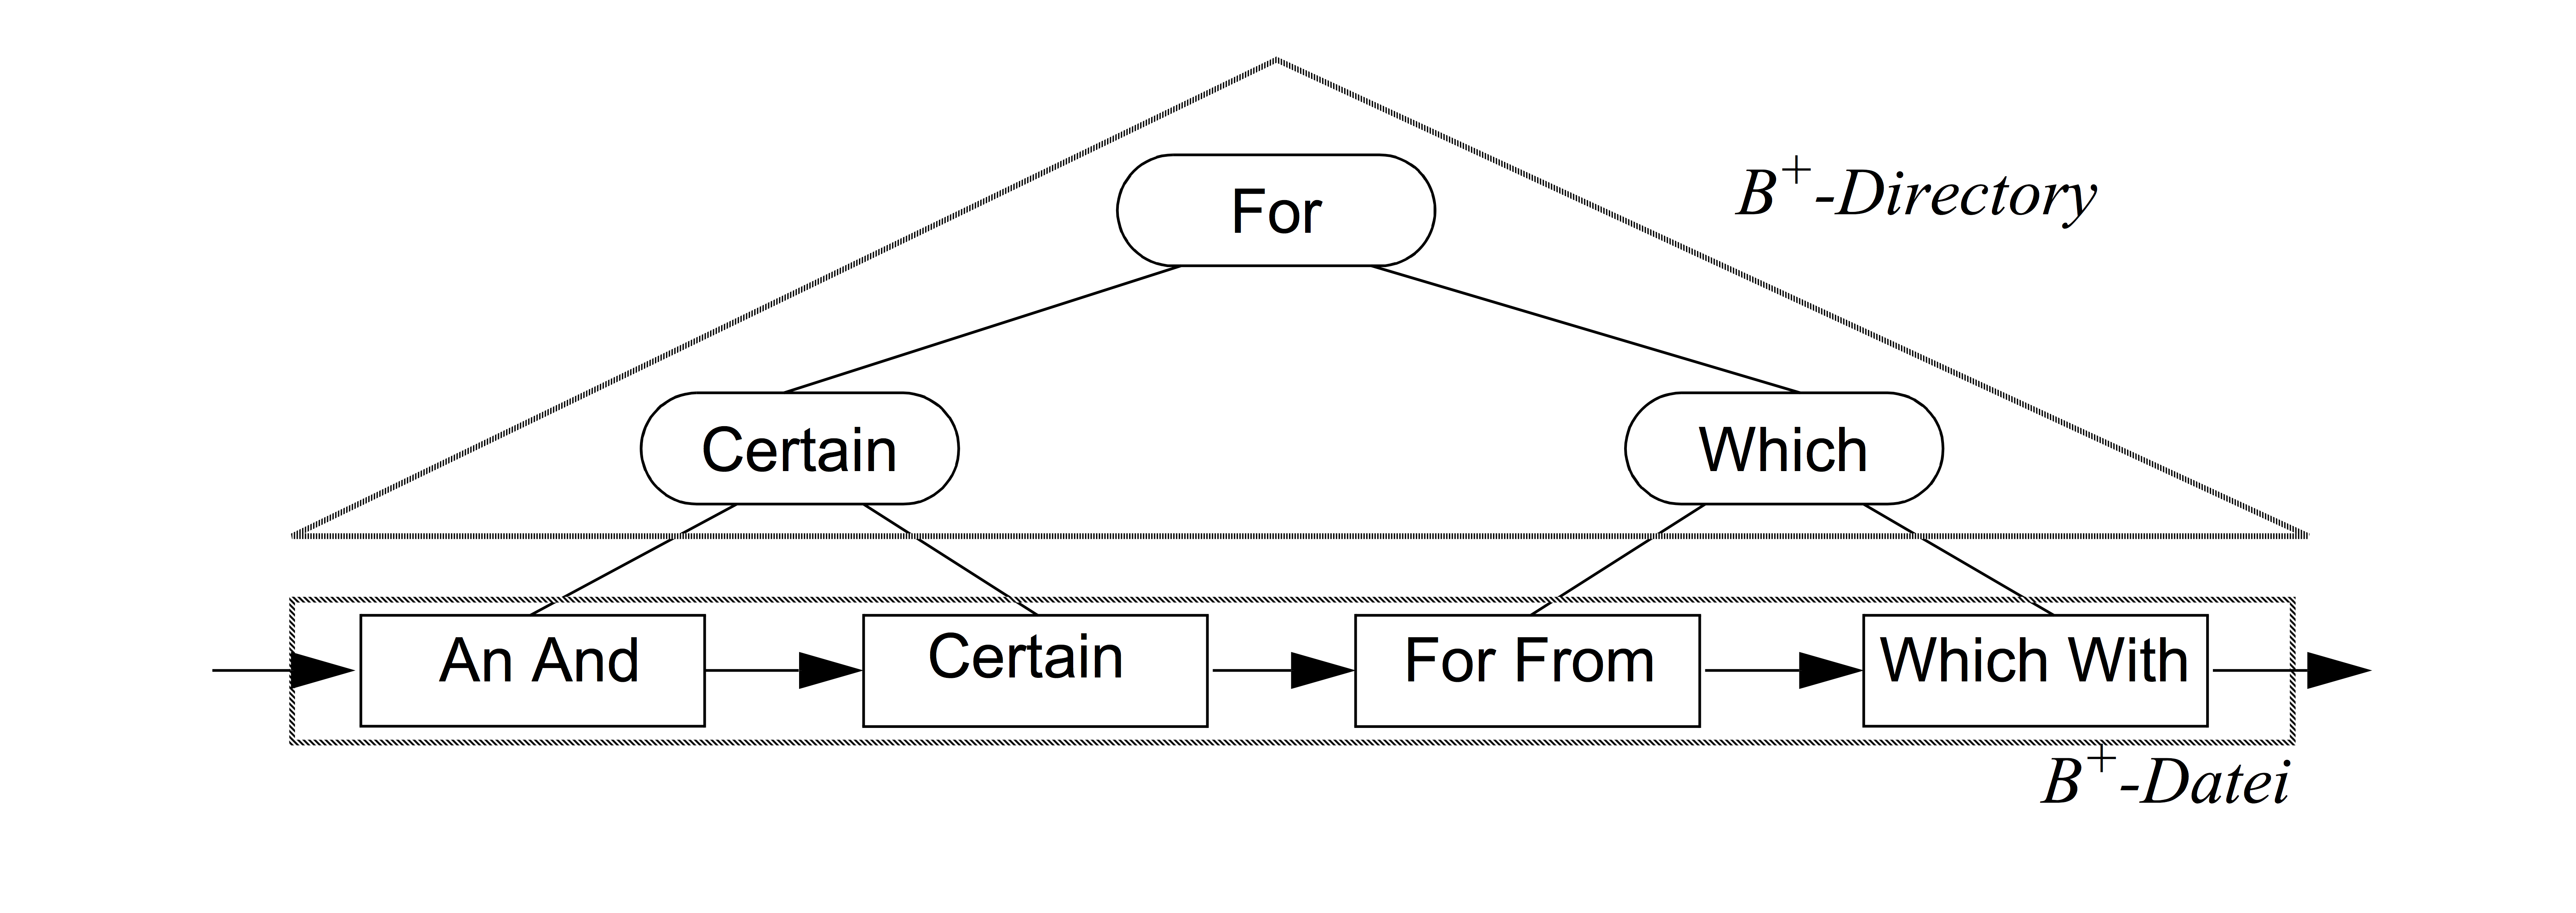
\includegraphics[width=1.0\textwidth]{pictures/b+baum.png}\\
  \caption[Ein B$^+$-Baum der Ordnung 2]{Ein B$^+$-Baum der Ordnung 2 \cite{Kriegel1994--2013}.}\label{fig:pic4}
\end{figure}
\noindent
Alle Blätter sind gemäß der Ordungsrelation verkettet, was durch die Pfeile auf Level 3 symbolisiert wird. Dieser B$^+$-Baum ermöglicht damit z.B. eine Bereichsanfrage vom Typ "`Lies die Informationen aller Datensätze im Bereich von \textbf{And} bis \textbf{For} aus"'. Dazu genügt es, einmal den Schlüssel \textbf{And} im Baum zu suchen und von dort aus den Zeigern auf der Blattebene zu folgen, bis entweder der Schlüssel \textbf{For} oder, wenn dieser nicht im Baum enthalten ist, ein Schlüssel mit einem lexikografisch größeren Wert erreicht ist. Solch eine Anfrage ist im B-Baum aus Abbildung \ref{fig:pic3} nicht möglich. Dort benötigt eine Anfrage nach allen Schlüsseln im Bereich von \textbf{B} bis \textbf{V} sechs rekursive Suchaufrufe, da es keine Möglichkeit gibt, die Nachbarknoten auf Blattebene zu erreichen. 
 
Neben der Bereichssuche zählt der höhere Verzweigungsgrad zu den wesentlichen Vorteilen des B$^+$-Baums gegenüber dem B-Baum. Tabelle \ref{tab:Trees} vergleicht die durchschnittlichen Laufzeiten für Einfügen, Suchen und Löschen in B-Bäumen und B$^+$-Bäumen.
\begin{center}
\begin{table}[htbp]
{\small
\begin{center}
\begin{tabular}[center]{lcccc}
\toprule
 & \textbf{Einfügen} & \textbf{Suchen} & \textbf{Löschen} & \textbf{Bereichssuche}\\
\midrule
\textbf{B-Baum} & $O(log (2t -1))$ & $O(log (2t -1))$ & $O(log (2t -1))$ & $\times$ \\
\midrule
\textbf{B$^+$-Baum} & $O(log (2t -1))$ & $O(log (2t -1))$ & $O(log (2t -1))$ & $O(log 2t-1)$\\
\bottomrule
\end{tabular}
\end{center}
} % end of tiny
\caption[Laufzeiten von Operationen auf Suchbäumen]{Laufzeiten von Operationen auf Suchbäumen.\label{tab:Trees}}
\end{table}
\end{center}
Daran wird deutlich, dass die Kosten für Einfügen, Suchen und Löschen in beiden Varianten vom Parameter \textit{t} abhängen. Da die inneren Knoten im B$^+$-Baum mehr Schlüssel enthalten als im B-Baum, wird der Baum breiter und flacher. Geht man davon aus, dass ein Zugriff auf einen inneren Knoten einem Plattenzugriff entspricht, wird deutlich, dass sich damit die Kosten für Einfügen, Suchen und Löschen gegenüber dem B-Baum reduzieren lassen.

Die sequentielle Verkettung der Blätter im B$^+$-Baum ermöglicht zudem eine Bereichssuche. Das ist ein immenser Vorteil gegenüber dem B-Baum, bei dem jeder für eine Bereichssuche jeder einzelne Datensatz mit Kosten von $O(log (2t -1))$ gesucht werden muss. Diese Kosten fallen beim B$^+$-Baum nur für den ersten Datensatz mit dem kleinsten Primärschlüssel an. Anschließend kann eine doppelt verkettete Liste traversiert werden.